\section{Implementation}%
\label{sec:implementation}

\subsection{Overview of the system}%
\label{sub:overview_of_the_system}


\begin{figure}[h]
     \centering
     \begin{subfigure}[h]{0.49\textwidth}
         \centering
         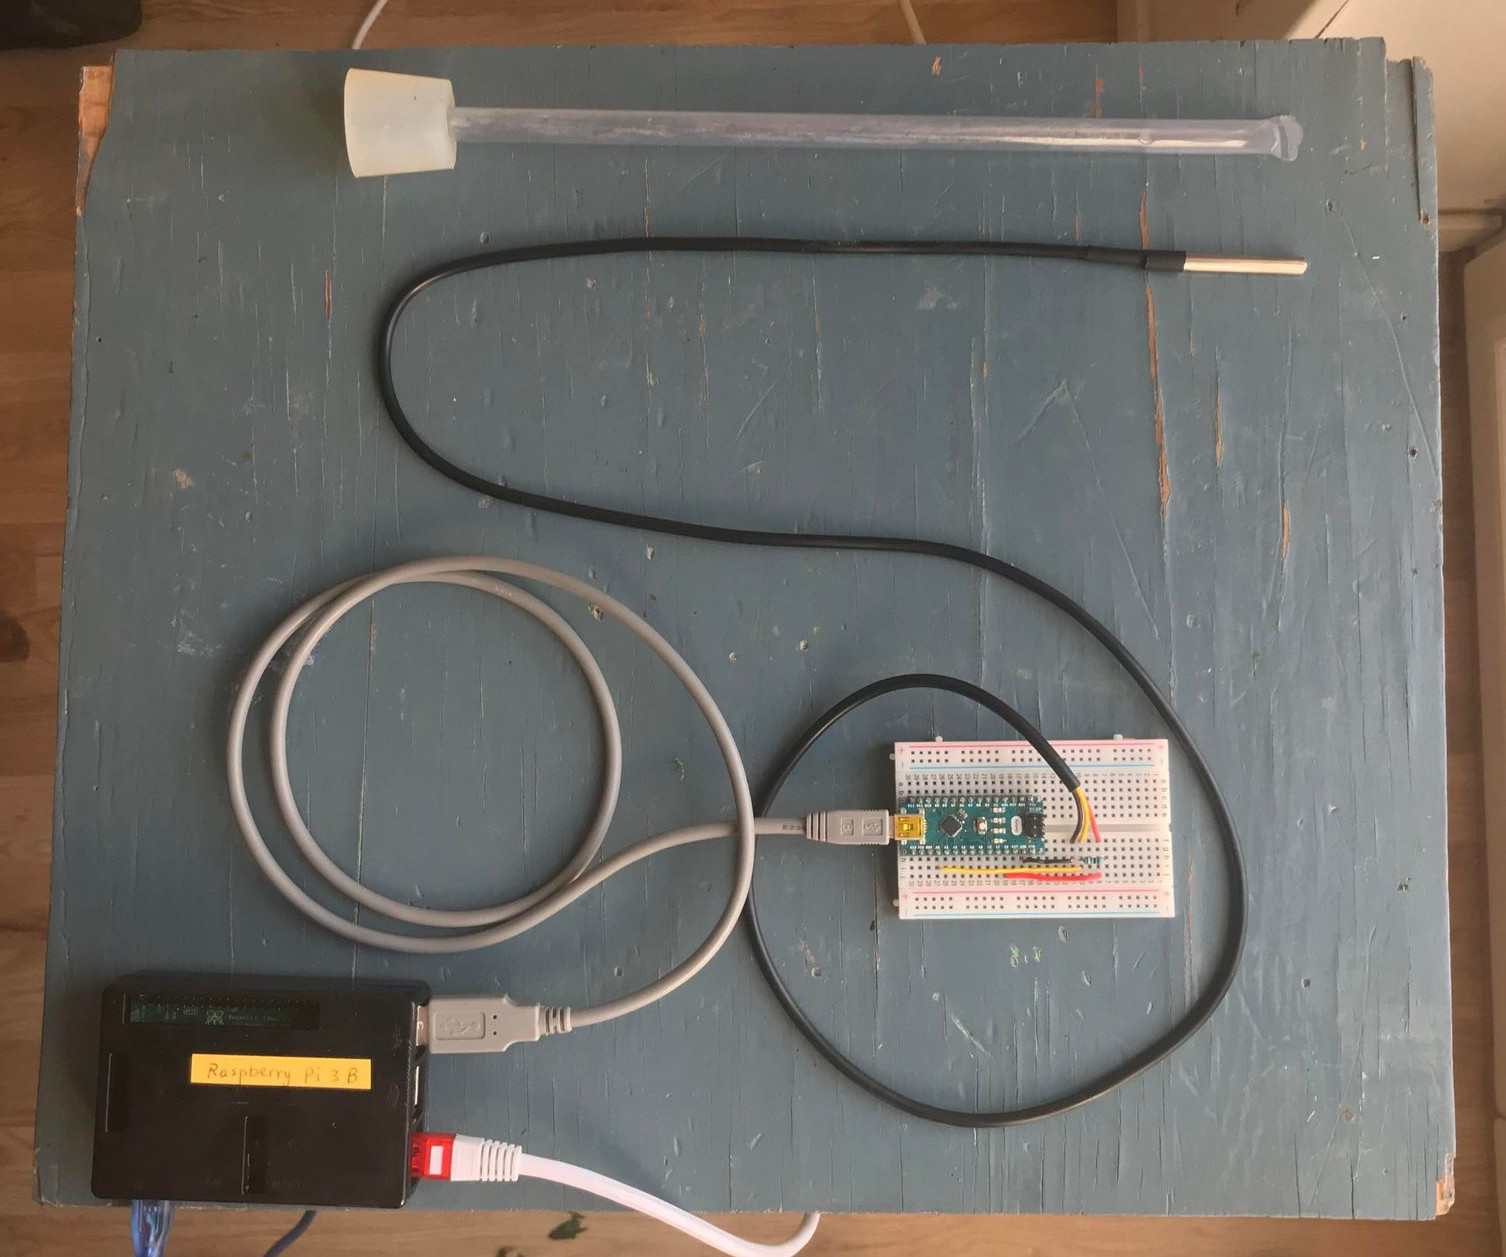
\includegraphics[width=\textwidth]{/home/auan/Project/Report/Images/part_overview.jpg}
         \caption{System overview}
         \label{fig:partsys}
     \end{subfigure}
     \hfill
     \begin{subfigure}[h]{0.41\textwidth}
         \centering
         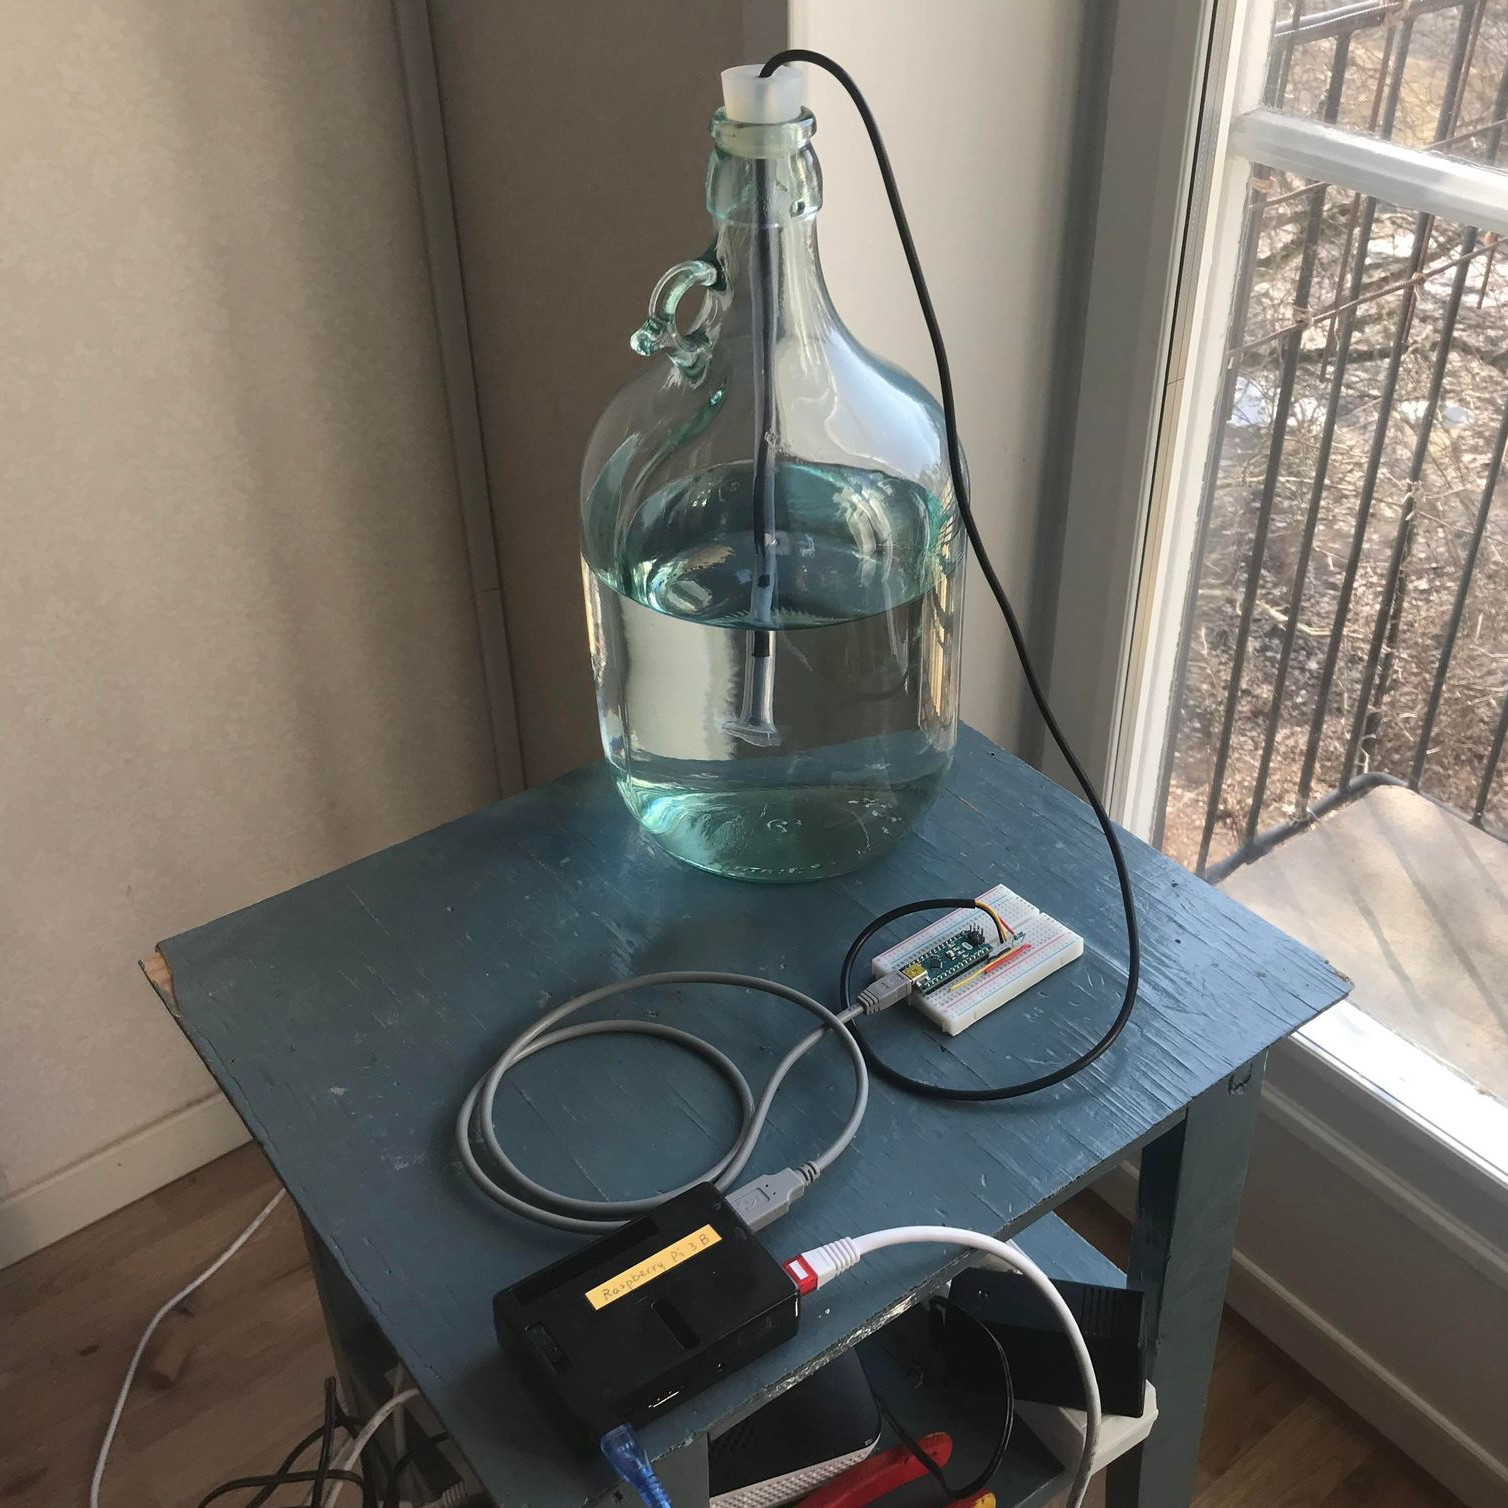
\includegraphics[width=\textwidth]{/home/auan/Project/Report/Images/full_overview.jpg}
         \caption{Submerged sensor}
         \label{fig:fullsys}
     \end{subfigure}
        \caption{The interconnected devices forms the monitoring system. As a safety precaution, the sensor is encapsulated in a food grade tube.}
        \label{fig:three graphs}
\end{figure}


%\begin{figure}[h]
  %\centering
  %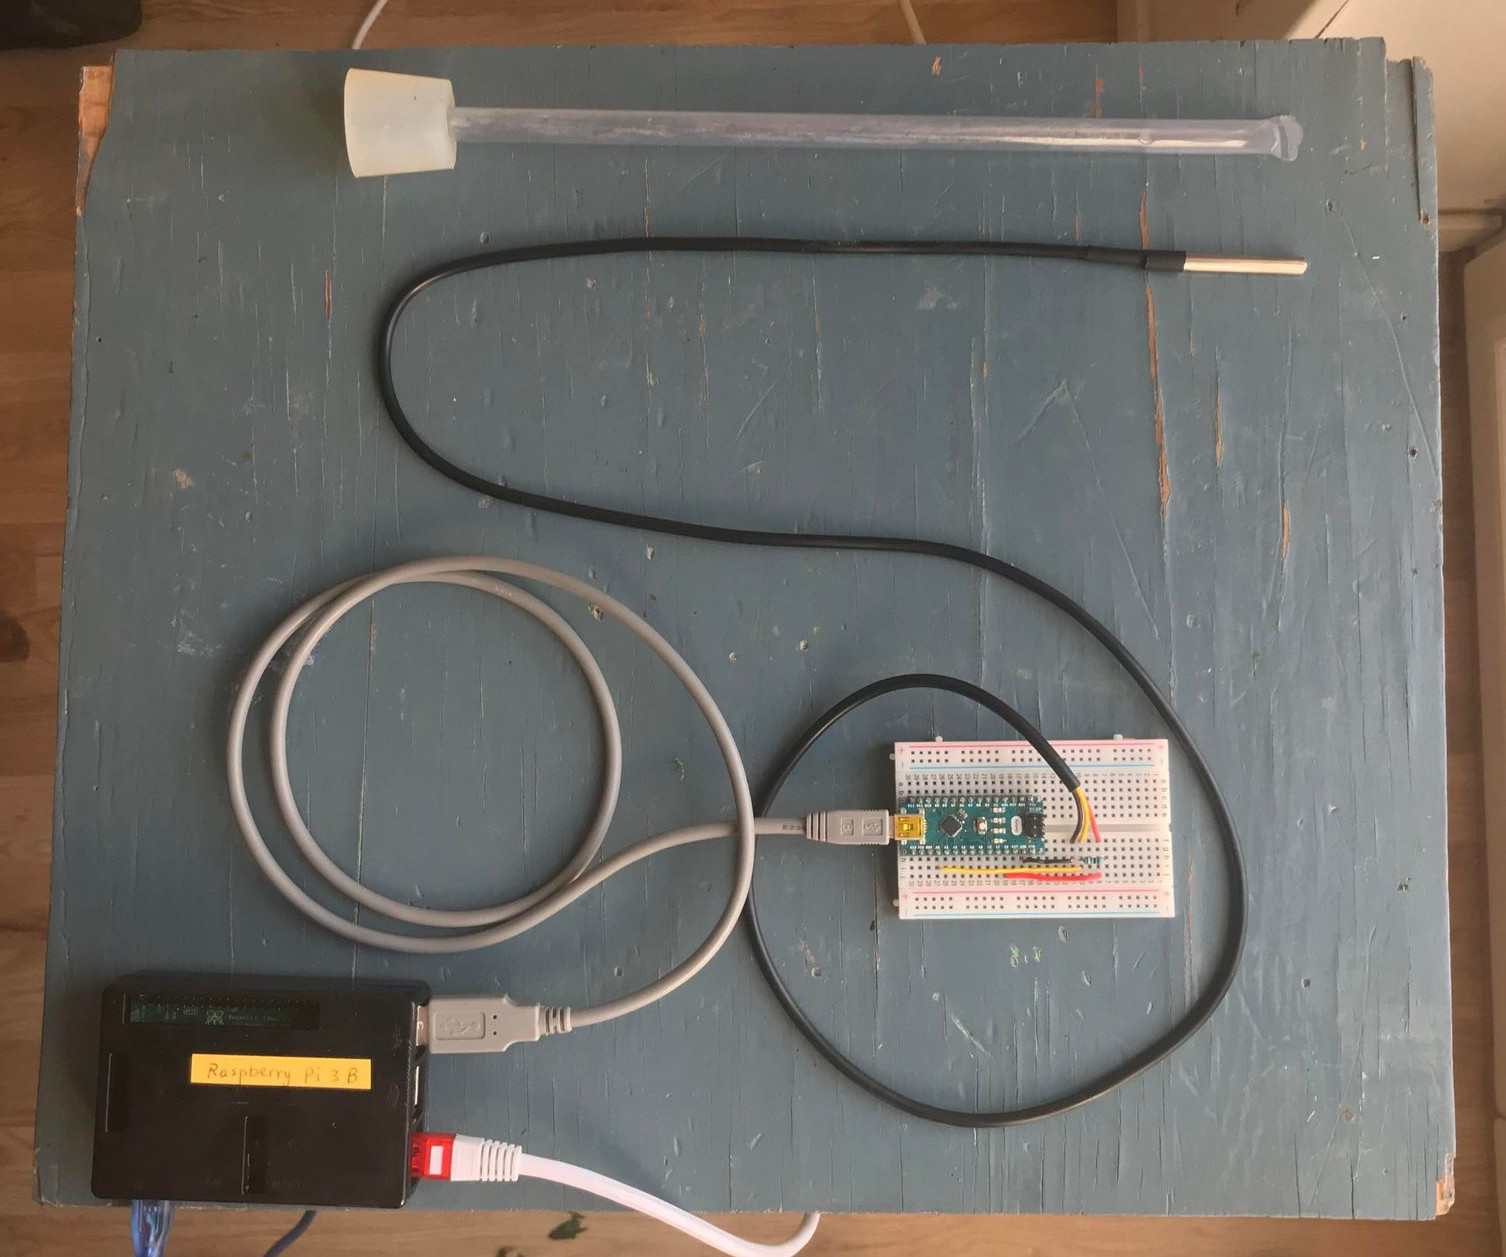
\includegraphics[width=0.6\textwidth]{/home/auan/Project/Report/Images/part_overview.jpg}
  %\caption{The system layout}
  %\label{fig:systemimg}
%\end{figure}
%The system overview can be seen in Figure \ref{fig:systemimg}. 
\begin{figure}[h]
  \centering
  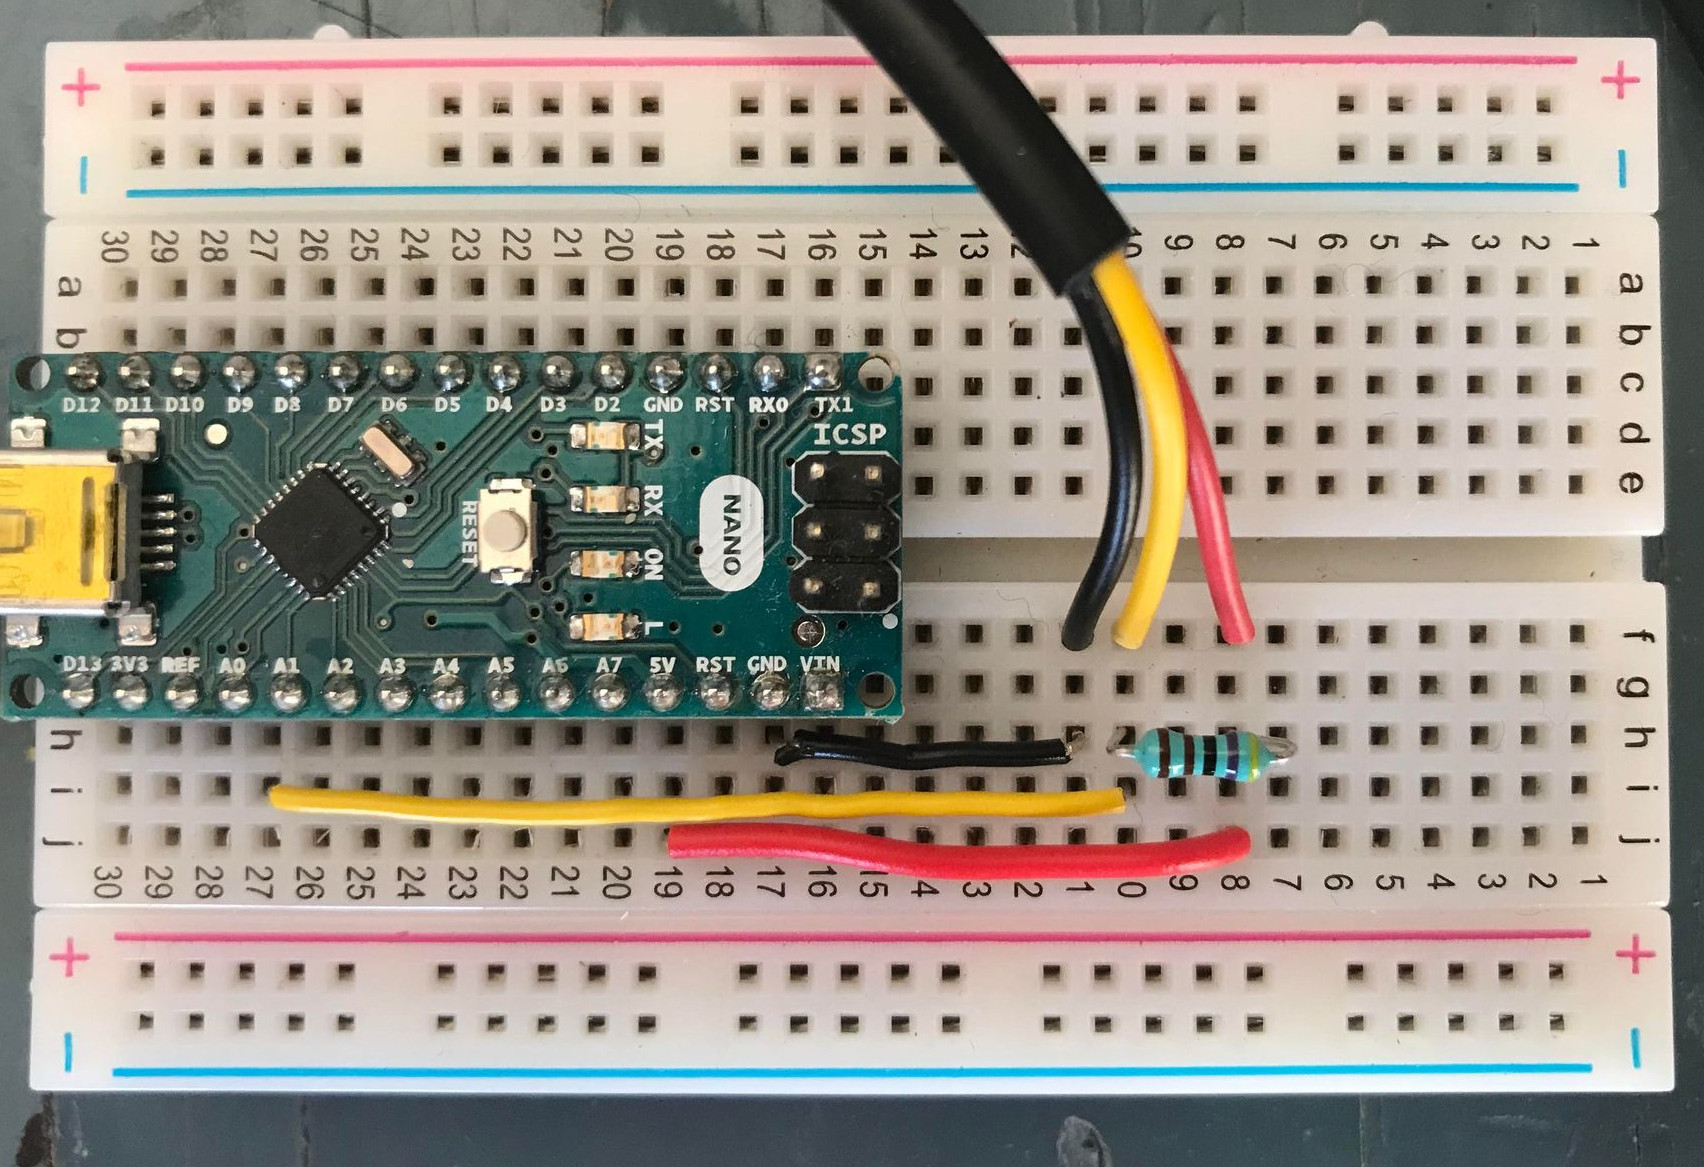
\includegraphics[width=0.6\textwidth]{/home/auan/Project/Report/Images/schematic.jpg}
  \caption{The Arduino and DS18B20 connected through a breadboard}
  \label{fig:breadboard}
\end{figure}

\newpage

\subsection{Hardware and components}%
\label{sub:hardware_and_components}
The software is written and compiled on a workstation grade Lenovo ThinkPad P14s Gen 2 with an AMD Ryzen 7 PRO 5850U.

The database and web application is hosted on a Raspberry Pi 3B which has a 64-bit ARM Cortex v8 processor running Arch Linux ARM \cite{RaspberryPiArch}. During the development, the RPi is connected to a router and accessed locally through the SSH protocol from the workstation.

The MCU is an Arduino Nano board equipped with the 32-bit ATmega328p microprocessor. It has an on-board serial to USB interface which is connected through a USB cable. This connection provides the binary files when flashing, UART data transfer as well as supplying 5V power for driving the board.

A DS18B20 temperature sensor is connected to the MCU through a breadboard. The reference voltage is and data signal is connected through a 4.7k$\Omega$ pull-up resistor.

\subsection{Software and development tools}%
\label{sub:software_and_development_tools}
\subsubsection{Neovim}%
\label{ssub:neovim}
Neovim is completely terminal based and it is possible to clone the configuration file (\verb|.init.vim|, often called a \textit{dotfile}) to the RPi and remotely access an IDE-like text editor without forwarding any graphics through the SSH connection \cite{DocumentationNeovim}.

Since the AVR library uses a lot of macros, it is handy to get help from an LSP. Neovim has built in LSP support and while the programmer might not use the \verb|clang| compiler for the actual compilation, it can be used with the \verb|ccls| language server.

\lstinputlisting[label={lst:ccls}, caption = {The hidden \texttt{.ccls} file in the project root directory sets the compiler flags of interest}]{/home/auan/Project/DS18B20_UART/.ccls}

\subsubsection{Cross-compilation}%
\label{ssub:cross_compilation}
In order efficiently utilize the workstation, the Embedded-C code is cross-compiled using the AVR-GCC toolchain. Given the information of what MCU model the program is going to run on, known as the target, GCC is able to compile accordingly. As with non-embedded C programs, GCC is able to optimize the code by setting the appropriate compiler flags. Optimizing the code has several gains such as creating faster programs that require less space.

\lstinputlisting[language=make, label={lst:makefile}, caption={GNU Makefile for compiling and flashing the program to the MCU}]{/home/auan/Project/DS18B20_UART/Makefile}

In Listing \ref{lst:makefile}, only the binary \verb|.elf| file from line 21 is flashed as a \verb|.hex| file on line 32. 

\subsubsection{Org-mode}%
\label{ssub:org_mode}
Org-mode is a text based software written in Emacs Lisp \cite{OrgMode}. It is highly extensible and can be customized in order to create TODO lists, schedule meetings and write journal entries in order to document the project work.

\subsubsection{AVR-GCC Toolchain}%
\label{ssub:avr_gcc_toolchain}
The code is compiled and uploaded to the MCU using a technique known as \textit{cross compilation} which utilizes the speed of a workspace computer in order to compile and upload the binary \verb|.hex| file. Compilation commands provided by the AVR-GCC toolchain \cite{GCCCompilersAVR} is called from a GNU Makefile which also handles hardware specific parameters such as CPU clock frequency, Baud rate and optimizer flags. 

\subsubsection{Git}%
\label{ssub:git}
Git, described by its man-page as \textit{the stupid content tracker} is a versioning tool originally created by Linus Torvalds \cite{git} when developing the Linux operating system. The whole project is stored locally within a git repository and hosted remotely by GitHub in order to synchronize the work between the Raspbery Pi and the workstation.
\subsubsection{VimTeX}%
\label{ssub:vimtex}
The report is written in \LaTeX and compiled using the Neovim VimTeX plug-in \cite{lervagVimTeX2022}.

\subsection{Implementation}%
\label{sub:implementation}

\subsubsection{UART drivers}%
\label{ssub:uart_drivers}
Calculating the correct register values, given the Baud rate, can be done directly from the file \verb|setbaud.h|. To enable the communication, the external interrupts, \verb|SEI()|, must be set in the C program. In Listing \ref{lst:uartreg} below
\begin{lstlisting}[caption={Enabling UART on the ATmega328p}, label={lst:uartreg}]
UBRR0H = UBRRH_VALUE;
UBRR0L = UBRUBRR0L = UBRRL_VALUE;

UCSR0B = (1 << RXEN0) | (1 << TXEN0) | (1 << RXCIE0) | (1 << TXCIE0);
\end{lstlisting}
the transfer and receive registers are also activated according to the ATmega328p datasheet \cite{atmega328p} where  
\begin{equation}
  UBRR = \frac{f_{osc}}{16\cdot BAUD} -1.
\end{equation}
Using a fixed clock frequency, it is possible to look up the rate of error given a set Baud rate. 
\begin{table}[h]
  \centering
  \caption{Baud and error rate}
  \label{tab:bauderr}
  \begin{tabular}{lccl}\toprule
  & \multicolumn{2}{c}{$f_{osc} = 16000000$ Hz}
  \\\cmidrule(lr){2-3}
  Baud & UBRRn  & Error \\\midrule
  9600 & 103 & 0.2\% \\
  14400 & 68 & 0.6\% \\
  57600 & 18 & 2.1\% \\\bottomrule
  \end{tabular}
\end{table}

In Table \ref{tab:bauderr}, the error rate for a Baud rate of 9600 produces is low and suffices since the small amounts of data is sent on an hourly basis. 

\subsubsection{DS18B20 drivers}%
\label{ssub:ds18b20_drivers}
The DS18B20 digital temperature sensor is manufactured by Maxim Integrated and the drivers used are based on Martin Thomas' modifications of Peter Dannegger's work (see credits in Appendix) on implementing the 1-wire library. 
\lstinputlisting[firstline=55,lastline=64, caption={The hex code instructions for the DS18B20 sensor defined as macros in \texttt{onewire.h}}, label={lst:onewire}]{~/Project/DS18B20_UART/inc/onewire.h}

While Maxim Integrated does not provide or support driver source code, it is possible to write the drivers from reading guides on how to interface the hardware \cite{DS18B20ProgrammableResolution}. The 1-Wire protocol has, as the name suggests, one data wire for receiving instructions defined in Listing \ref{lst:onewire} and transferring the requested data. The schematic and flow of data is visualized in Figure \ref{fig:sensorschem}. The data is written to the scratchpad and converted from a 12-bit two's complement binary resolution into a decimal floating point value with 0.0625 precision.

\begin{figure}[h]
  \centering
  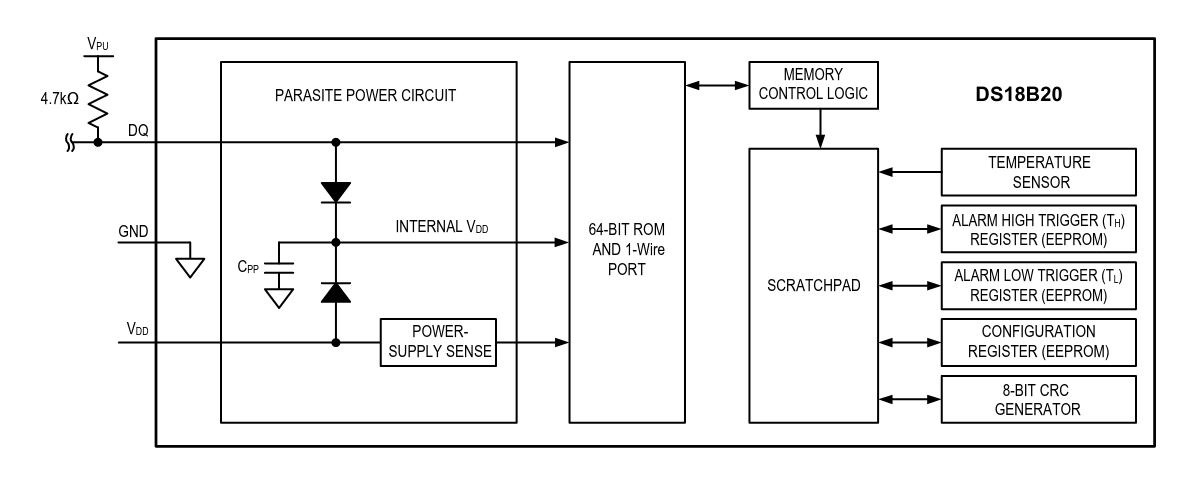
\includegraphics[width=0.8\textwidth]{/home/auan/Project/Report/Images/DS18B20_schem.png}
  \caption{Schematic of the DS18B20 sensor \cite{DS18B20ProgrammableResolution}}
  \label{fig:sensorschem}
\end{figure}
\subsubsection{MongoDB}%
\label{ssub:mongodb}
MongoDB is an open source document database suitable for storing time-series data. This acts as the web application back-end and can also store configuration options set by the user. The database can be set up to run a daemonized process, which allows the user to get or set data whenever the server is powered on. Using the Python module PyMongo \cite{PyMongo}, it is possible to insert entries using JSON formatting.

\subsubsection{Systemd service}%
\label{ssub:systemd_service}
Many Linux distributions use the Systemd init daemon as the first process booting and spawning other processes \cite{SystemdArchWiki}. While many crucial programs runs in the background by Systemd as default, it is quite straightforward to add a another service that in this case runs the Python temperature reading script. Systemd has several options to restart the service on failure, start without the need to login and redirect \verb|stdout| to the OS log called the \textit{Linux Journal}. This simplifies tracking how often the service behaves unexpectedly during long timespans.

\begin{lstlisting}[caption={The systemd service managing data collection}, label={systemd}]
[Unit]
# Human readable unit name
Description=Reads serially from '/dev/ttyUSB*' and puts in MongoDB

[Service]
# Command that executes script
ExecStart=/usr/bin/python /home/alarm/Project/serial_temp_to_db.py
# Redirect print() to the Linux journal
Environment=PYTHONUNBUFFERED=1
# Able to notify that the service is ready
Type=notify
Restart=always

[Install]
# Start service at boot
WantedBy=default.target
\end{lstlisting}


\subsubsection{Plotly Dash web application}%
\label{ssub:plotly_dash_web_application}
The web application consists of
\begin{enumerate}
  \item A live graph showing the specified range of most recent data points. It is updated by a callback function listening to a timer.
  \item A graph showing the historical data of measurements. The user can pick start and stop times from in the span of the registered dates in the database. The data is updated if the page is refreshed.
  \item The user can set alarm levels which sends and alert email if a drastic temperature drop is detected.
\end{enumerate}

Dash is an open source data visualization framework that runs in a web application. It is maintained by Plotly and build upon using their graphing software with the same name.

\begin{lstlisting}[language=python, caption={Pseudocode showing the structure of a Plotly Dash app}, label={lst:dash}]
  import dash dependencies
  import modules

  external_stylesheets = ['stylesheet.css']
  
  app = dash.Dash(__name__, external_stylesheets=external_stylesheets)

  # The application layout
  app.layout = html.Div(children =[
      html.H1('Large Heading'),
      html.H3('Smaller Heading'),
      html.Div([
          dcc.Graph(id='graph-id', animate=False),
          dcc.Interval(
              id='interval-component',
              interval=1*UPDATE_INTERVAL
              )
          ])
      )

# Callback function decoration
@app.callback(
    Output("update-figure", "figure"),
    Input("interval-component", "n_intervals"),
)

# Figure manipulation
def update_figure():
  return figure

if __name__ == '__main__':
    app.run_server(debug=True, host="0.0.0.0")
\end{lstlisting}


Each website object can be decorated with a callback function that either updates due to a time interval or through user interaction. In the example Listing \ref{lst:dash}, the graph is updated using a timer interval but can be changed to text fields or interactive clickable elements. The application is running as a server on port \verb|8080| and the address \verb|0.0.0.0| allows any unit on the local network to access the application web page by specifying the IP address followed by the correct port number.  Since Dash is well documented for using Pandas, the data is loaded into a dataframe object which allows many ways of manipulation in areas such as statistics and signal processing. The data ordered by a time stamp, and is sorted in natural order, where the start and stop date can be chosen by the using a date picker.

\subsubsection{Gmail API alert}%
\label{ssub:gmail_api_alert}
One of the brewers worst enemies is oxidation. For homebrewers, it is very common to use an airlock that lets carbon dioxide escape when it reaches a certain over-pressure. A problem with this is caused by the exact opposite phenomena -- when the beer and gas volume shrinks due to decreasing temperature which leads to oxygen entering through back pressure. An alert feature is implemented for storing fermentation vessels in an environment with fluctuating temperature and uses a parameter set by the user to the define how sensitive the alerting mechanism is to temperature drops. If a large enough drop is detected, the Systemd service uses the web based Gmail API to send an alert.
